\documentclass[answers]{exam}

\usepackage{amsmath}
\usepackage{amssymb}
\usepackage{geometry}
\usepackage{venndiagram}
\usepackage{graphics}
\usepackage{graphicx}
\usepackage{tikz}
\usepackage{listings}
\usepackage{float}

% Header and footer.
\pagestyle{headandfoot}
\runningheadrule
\runningfootrule
\runningheader{EE/CE 468/468 Mobile Robotics}{Homework 2}{Fall 2023}
\runningfooter{}{Page \thepage\ of \numpages}{}
\firstpageheader{}{}{}

\boxedpoints
\printanswers

\newcommand{\uvec}[1]{\boldsymbol{\hat{\textbf{#1}}}}
\newcommand\union\cup
\newcommand\inter\cap
\newcommand\ul\underline
\newcommand\ol\overline

\title{Assignment 2\\ EE/CE 468/468 Mobile Robotics\\ Habib University -- Fall 2023}
\author{Ali Asghar Yousuf \\ Muhammad Azeem Haider }  % replace with your ID, e.g. oy02945
\date{\today}

\begin{document}
\maketitle

\begin{questions}
    \question Problem 2
    \question Problem 3
    \subsection*{Code}

    \begin{lstlisting}
    function [v, w] = pidPathFollower(Pose, WayPoints)
        persistent n;
        persistent k;
        if (isempty(n))
            n = 2;
            k = 0;
        end
        % Completed the path
        if n > length(WayPoints)
            v = 0;
            w = 0;
        else
        x = Pose(1);
        y = Pose(2);
        phi = Pose(3);
        R = [cos(phi) sin(phi); -sin(phi) cos(phi)];
        % WayPointsPhi = [0 pi/2 pi 3*pi/2];

        xref = WayPoints(n, 1);
        yref = WayPoints(n, 2);
        phiref = WayPoints(n, 3);

        ep = R*([xref; yref]-[x; y]);
        xe = ep(1);
        ye = ep(2);
        d = sqrt(ye^2 + xe^2);
        eps = 0.1;

        phie = phiref - phi;
        if d < eps
            n = n + 1;
        end
        % v = 0.2*xe + 0.1;
        % k = 60*(ye) + 0.08*sin(-phie);  
        % w = v*k;

        v = 0.8*xe + 0.8;
        k = 60*(ye) + 0.15*sin(-phie);
        w = v*k;

        end
    end
    \end{lstlisting}

    \subsection*{Waypoint Tracking}
    \begin{figure}[H]
        \centering
        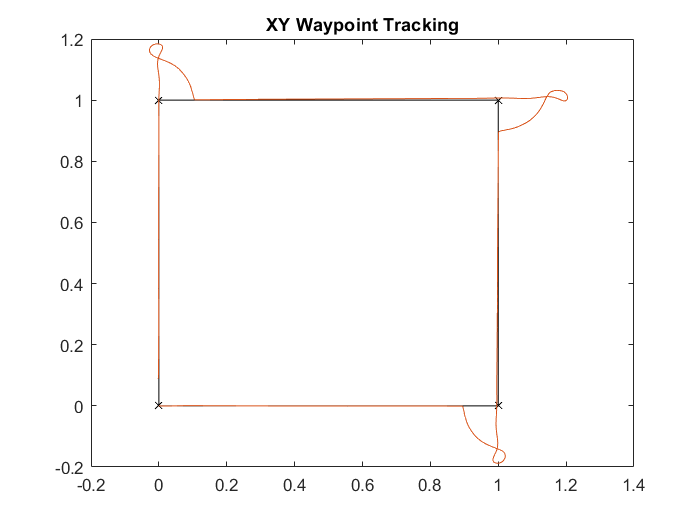
\includegraphics[width=0.8\textwidth]{images/3.png}
        \caption{PID Path Follower}
        \label{fig:my_label}
    \end{figure}

    \question Problem 4
    \subsection*{Waypoint Tracking}
    \begin{figure}[H]
        \centering
        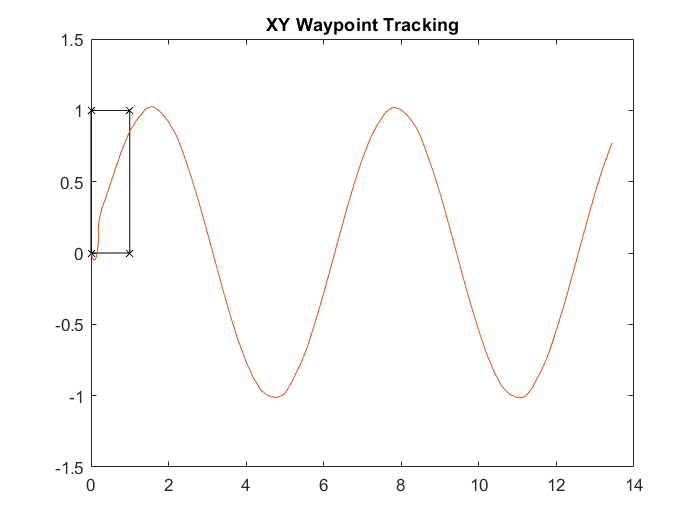
\includegraphics[width=0.8\textwidth]{images/4-wave.png}
        \caption{Wave}
        \label{fig:my_label}
    \end{figure}

    \begin{figure}[H]
        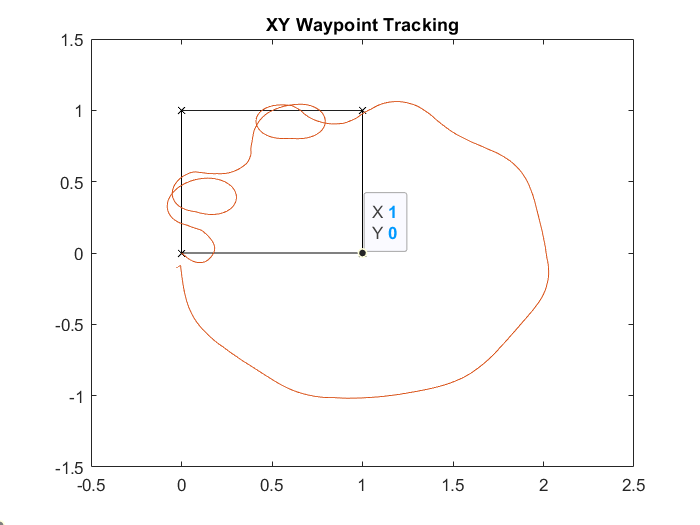
\includegraphics[width=0.5\textwidth]{images/4-circle-r1.png}
        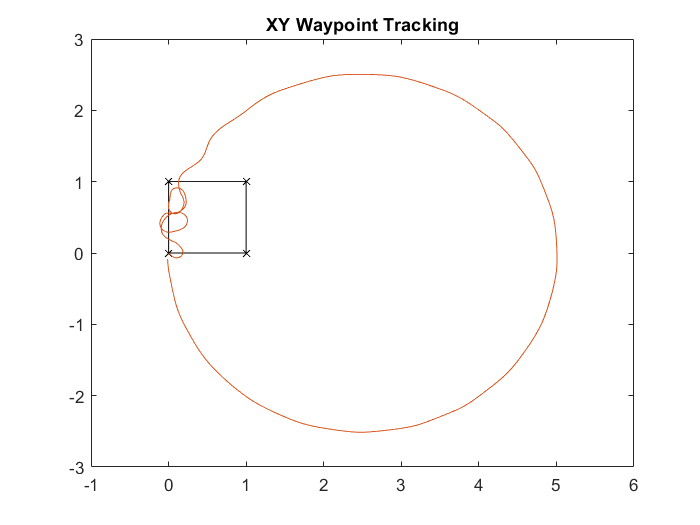
\includegraphics[width=0.5\textwidth]{images/4-circle-r2.5.png}
        \caption{Circle}
        \label{fig:my_label}
    \end{figure}

\end{questions}

\end{document}